\documentclass[../Cours.tex]{subfiles}

\begin{document}
\chapitre{Horaires et durées}

\partie{Horaires}

\vocabulaire{Une année correspond à la durée d'un tour complet de la Terre autour du Soleil.}

\begin{center}
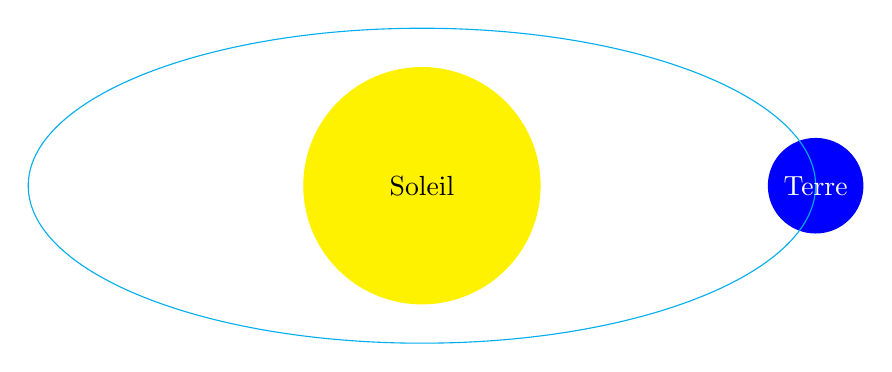
\begin{tikzpicture}
    \draw[yellow, fill=yellow] (0,0) circle (1.5);
    \node at (0,0) {Soleil};
    \draw[blue, fill=blue] (5,0) circle (0.6);
    \draw[cyan] (0,0) ellipse (5 and 2);
    \node[white] at (5,0) {Terre};
\end{tikzpicture}
\end{center}

\remarque{Année légale : 365 jours/366 jours\\Année tropique : 365,25 jours}

\vocabulaire{1 jour = 24 heures\\1 heure = 60 minutes\\1 minute = 60 secondes}

\remarque{1 jour = 8640 secondes\\1 heure = 3600 secondes}

\definition{Une horaire est un ou plusieurs nombres (en général représentant les heures et les minutes) permettant de décrire le temps écoulé depuis le début du jour (minuit).}

\begin{listedexemples}
    \item 11h42 $\longrightarrow$ onze heures et quarante-deux minutes
    \item 22h55 $\longrightarrow$ vingt-deux heures cinquante-cinq minutes
    \item $12:05$ pm $\longrightarrow$ midi cinq
\end{listedexemples}

\clearpage
\remarque{Format de l'heure anglaise
\begin{multicols}{4}
\begin{itemize}\small
    \item 00h $\rightarrow$ 12:00 am
    \item 01h $\rightarrow$ 01:00 am
    \item 02h $\rightarrow$ 02:00 am
    \item 03h $\rightarrow$ 03:00 am
    \item 04h $\rightarrow$ 04:00 am
    \item 05h $\rightarrow$ 05:00 am
    \item 06h $\rightarrow$ 06:00 am
    \item 07h $\rightarrow$ 07:00 am
    \item 08h $\rightarrow$ 08:00 am
    \item 09h $\rightarrow$ 09:00 am
    \item 10h $\rightarrow$ 10:00 am
    \item 11h $\rightarrow$ 11:00 am
    \item 12h $\rightarrow$ 12:00 pm
    \item 13h $\rightarrow$ 01:00 pm
    \item 14h $\rightarrow$ 02:00 pm
    \item 15h $\rightarrow$ 03:00 pm
    \item 16h $\rightarrow$ 04:00 pm
    \item 17h $\rightarrow$ 05:00 pm
    \item 18h $\rightarrow$ 06:00 pm
    \item 19h $\rightarrow$ 07:00 pm
    \item 20h $\rightarrow$ 08:00 pm
    \item 21h $\rightarrow$ 09:00 pm
    \item 22h $\rightarrow$ 10:00 pm
    \item 23h $\rightarrow$ 11:00 pm
\end{itemize}
\end{multicols}
}

\partie{Dates}

\convention{Forme simplifiée : Jour/Mois/Année\\
Forme développée : le [Nom du jour] Jour [Nom du mois] Année}

\exemple{Aujourd'hui :
\begin{itemize}
    \item Forme simplifiée : 19/01/2023
    \item Forme développée : le jeudi 19 janvier 2023
\end{itemize}}

\vocabulaire{\vspace{-3ex}
\begin{itemize}
    \item Un millénaire = 1000 ans
    \item Un siècle = 100 ans
    \item Une décennie = 10 ans
\end{itemize}
}

\souspartie{Fuseaux horaires}

\paragraphe{rouge}{Norme}{ISO 8601}
\exemple{Le 2 mai 2022 à 13h57min12s en France métropolitaine : 2022-05-02T13:57:12+02:00\\
\begin{center}
\begin{tikzpicture}
    \node at (0,0) {2022~-~05~-~02~T~13~:~57~:~12~+~02~:~00};
    \node[rouge] at (-3.6,-0.5) {année};
    \node[rouge] at (-2.3,-0.5) {mois};
    \node[rouge] at (-1.2,-0.55) {jour};
    \node[rouge] at (0,-1) {heures}; 
    \draw[Latex-,rouge] (-0.1,-0.25) -- (-0.1,-0.8);
    \node[rouge] at (0.8,-0.5) {minutes};
    \node[rouge] at (1.8,-1) {secondes}; 
    \draw[Latex-,rouge] (1.7,-0.25) -- (1.7,-0.8);
    \node[vert] at (4,-0.5) {fuseau horaire}; 
    \draw[vert] (2.25,-0.3) rectangle (3.8,0.3);
\end{tikzpicture}
\end{center}
}

\definition{La surface de la Terre est découpée en plusieurs zones appelées \emph{fuseaux horaires}. Chaque zone a une heure locale différente, définie par rapport au UTC (Temps Universel Coordonné), originellement défini par rapport au méridien de Greenwich.}

\notation{<< UTC+04:00 >> signifie << 4 heures de plus par rapport au méridien de Greenwich >>.}

\remarque{La France est le pays qui a le plus de fuseaux horaires : 13.
\begin{itemize}
    \item[$\blacksquare$] UTC−10:00 — La plus grande partie de la Polynésie française
    \item[$\blacksquare$] UTC−09:30 — Îles Marquises
    \item[$\blacksquare$] UTC−09:00 — Îles Gambier
    \item[$\blacksquare$] UTC−08:00 — Île Clipperton
    \item[$\blacksquare$] UTC−04:00 — Guadeloupe, Martinique, Saint-Barthélemy et Saint-Martin,
    \item[$\blacksquare$] UTC−03:00 — Guyane et Saint-Pierre-et-Miquelon
    \item[$\blacksquare$] UTC+01:00 — France métropolitaine et Corse
    \item[$\blacksquare$] UTC+03:00 — Mayotte
    \item[$\blacksquare$] UTC+04:00 — La Réunion, les îles Éparses de l'océan Indien et l'archipel Crozet
    \item[$\blacksquare$] UTC+05:00 — Îles Kerguelen, îles Saint-Paul et Nouvelle-Amsterdam
    \item[$\blacksquare$] UTC+10:00 — Terre Adélie
    \item[$\blacksquare$] UTC+11:00 — Nouvelle-Calédonie
    \item[$\blacksquare$] UTC+12:00 — Wallis et Futuna
\end{itemize}
En heure d'été, la France métropolitaine est en UTC+02:00 au lieu de UTC+01:00.
}

\exemple{Il est 15h45 sur l'île de la Réunion, quelle heure est-il en Guyane française ?\\
\begin{center}\color{noir}
\begin{tikzpicture}
    \node at (0,0) {Greenwich};
    \node at (-5,0) {Guyane};
    \node at (6,0) {Île de la Réunion};
    \node at (0,-0.5) {UTC+00:00};
    \node at (-5,-0.5) {UTC-03:00};
    \node at (6,-0.5) {UTC+04:00};
    \node at (6,-1.3) {15h45};
    \draw[-Latex] (6,-1.7) arc(0:-180:2.7 and 0.8) node[midway,below]{-4h};
    \node at (0,-1.3) {11h45};
    \draw[-Latex] (-0.5,-1.7) arc(0:-180:2.1 and 0.8) node[midway,below]{-3h};
    \node at (-5,-1.3) {08h45};
\end{tikzpicture}
\end{center}
}

\clearpage
\partie{Conversions}
\souspartie{hh:mm:ss}

\methode{Pour convertir les secondes en minutes et secondes, on effectue une division euclidienne par 60.}
\exemple{Convertir \qty{1245}{\second} en minutes et secondes}

\begin{center}
    \begin{tikzpicture}
        \node at (0,0) {\opidiv[displayintermediary=all,dividendbridge]{1245}{60}};
        \draw[vert] (-0.4,-1.6) rectangle (0.5,-1.05);
        \draw[rouge] (0.9,0.5) rectangle (1.7,0.95);
        \node[anchor=west] at (3,0) {\qty{1245}{\second} $=$ {\color{rouge}20} minutes et {\color{vert}45} secondes};
    \end{tikzpicture}
\end{center}

\methode{Pour convertir les secondes en heures, minutes et secondes, on effectue deux divisions euclidiennes successive par 60.}
\exemple{Convertir \qty{10345}{\second} en heures, minutes et secondes}

\begin{center}
    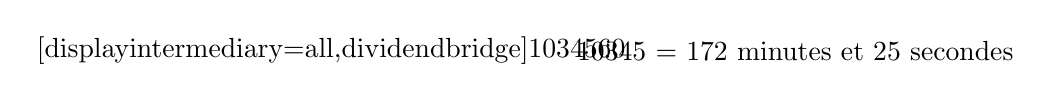
\begin{tikzpicture}
        \node at (0,0) {\opidiv[displayintermediary=all,dividendbridge]{10345}{60}};
        \node[anchor=west] at (3,0) {\qty{10345}{\second} $=$ 172 minutes et 25 secondes};
    \end{tikzpicture}
\end{center}
\begin{center}
    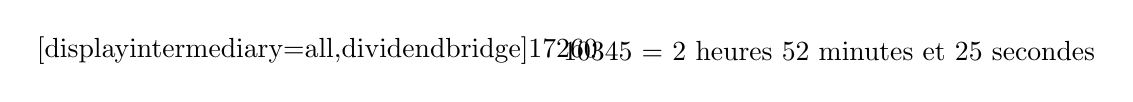
\begin{tikzpicture}
        \node at (0,0) {\opidiv[displayintermediary=all,dividendbridge]{172}{60}};
        \node[anchor=west] at (3,0) {\qty{10345}{\second} $=$ 2 heures 52 minutes et 25 secondes};
    \end{tikzpicture}
\end{center}

\methode{Dans l'autre sens, on multiplie les heures par 3600, et les minutes par 60, afin d'obtenir le nombre de secondes.}
\exemple{Combien y a-t-il de secondes dans 5h25min13s ?}

\begin{align*}
    \mbox{5h25min13s} &= 5 \times 3600 + 25 \times 60 + 13 \\
    &= 18000 + 1500 + 13 \\
    &= \qty{19513}{\second}
\end{align*}

\souspartie{Vitesse}

\formule{La vitesse moyenne $v$ d'un objet ayant parcouru une distance $d$ sur un laps de temps $t$ est : 
\[ \mbox{vitesse} = \frac{\mbox{distance}}{\mbox{temps}} \hspace{3cm} v = \frac{d}{t} \hspace{0.5cm} \mbox{(abrégé)} \]}

\convention{On exprime généralement la vitesse en kilomètre par heure (\unit{\kilo\metre\per\hour}) ou en mètre par seconde (\unit{\metre\per\second}).}

\methode{Pour convertir les \unit{\metre\per\second} en \unit{\kilo\metre\per\hour} :
    \begin{center}\color{noir}
        \begin{tikzpicture}
            \node at (-3,0) {\unit{\metre\per\second}};
            \node at (3,0) {\unit{\kilo\metre\per\hour}};
            \draw[-Latex] (3,-0.5) arc(0:-180:3 and 0.8) node[midway,below]{$\div \num{3.6}$};
            \draw[-Latex] (-3,0.5) arc(180:0:3 and 0.8) node[midway,above]{$\times \num{3.6}$};
        \end{tikzpicture}
    \end{center}
}

\begin{listedexemples}
    \item $\qty{10}{\metre\per\second} = \qty{36}{\kilo\metre\per\hour}$
    \item $\qty{72}{\kilo\metre\per\hour} = \qty{20}{\metre\per\second}$
    \item $\qty{340}{\metre\per\second} = $
    \item $\qty{130}{\kilo\metre\per\hour} = $
\end{listedexemples}

\clearpage
\EXERCICES 
\begin{questions}
    \exercice
    \begin{multicols}{3}
        \questionX 2h35 + 4h43 = 
        \questionX 6h28 + 9h12 = 
        \questionX 8h37 + 9h12 = 
    \end{multicols}

    
    \exercice
    \question Si un film commence à 17h29 et dure 2 heures et 15 minutes, à quelle heure se termine-t-il ?
    \question Si une personne part de chez elle à 6h14 et met 1 heure et 32 minutes pour arriver au travail, à quelle heure arrive-t-elle ?
    \question Si un train part à 12h52 et met 5 heures et 12 minutes pour arriver à destination, à quelle heure arrive-t-il ?
    \question Un avion décolle à 18h45 et le vol dure 8h45, à quelle heure arrive-t-il ?
    

    \exercice
    \question Si le 13 mars tombe un lundi, quel jour est-il le 1er avril ?
    \question Cette année Pâques tombe le 9 avril 2023. Quel jour sera le jeudi de l'Ascension ?
    \question Le 1er janvier 2023 est un dimanche. Quel jour sera le 1er janvier 2024 ?

    \exercice 
    \question Il est 17h45 à Tokyo (UTC+09:00). Quelle heure est-il au même moment à Helsinki (UTC+02:00) ?
    \question Il est 23h34 à Santiago (UTC-04:00). Quelle heure est-il à New Dehli (UTC+05:30) ?
    \question Il est 03:05 à Bangkok (UTC+06:00). Quelle heure est-il à Saint-Marin (UTC+02:00) ?

    \exercice Un avion est parti de Varsovie à 06h05 (UTC+01:00) et a pour destination Montréal (UTC-05:00), le trajet dure 12h00. À quelle heure l'avion arrive-t-il à destination ?

    \exercice Convertir en hh:mm:ss
    \begin{multicols}{3}
        \questionX \qty{81702}{\second}
        \questionX \qty{17384}{\second}
        \questionX \qty{86400}{\second}
    \end{multicols}

    \exercice Combien y a-t-il de secondes dans...
    \begin{multicols}{3}
        \questionX 3h52min41s
        \questionX 12h00min06s
        \questionX 22h05min17s
    \end{multicols}

    \exercice Convertir les vitesses (\unit{\metre\per\second} $\longrightarrow$ \unit{\kilo\metre\per\hour} ou \unit{\kilo\metre\per\hour} $\longrightarrow$ \unit{\metre\per\second})
    \begin{multicols}{3}
        \questionX \qty{108}{\kilo\metre\per\hour} =
        \questionX \qty{83}{\metre\per\second} = 
        \questionX \qty{98}{\metre\per\second} = 
    \end{multicols}

    \exercice Le Concorde est un avion de ligne \emph{supersonique} qui pouvait relier l'Europe et l'Amérique en allant à une vitesse de croisière de \qty{2145}{\kilo\metre\per\hour}.

    \question Donner cette vitesse en \unit{\metre\per\second}.
    \question On peut aussi affirmer que $\qty{2145}{\kilo\metre\per\hour} = \qty{2.02}{Ma}$, où << Ma >> est l'abréviation de << Mach >>, la vitesse du son. Cela signifie donc que le Concorde avait une vitesse de croisière égale à \num{2.02} fois la vitesse du son. \textbf{En déduire la valeur de la vitesse du son.}
    \question Le Concorde permettait de relier Paris à New York en 3h30. S'il décolle de Paris à 17h30 (heure de Paris : UTC+02:00), à quelle heure arrive-t-il à New York (UTC-04:00) ?
\end{questions}

\clearpage
\CORRECTIONS
\begin{questions}
    \exercice
    \question 2h35 + 4h43 = 6h78 = 7h18
    \question 6h28 + 9h12 = 15h42
    \question 8h37 + 9h12 = 17h49    
\end{questions}

\end{document}